\documentclass[1p]{elsarticle_modified}
%\bibliographystyle{elsarticle-num}

%\usepackage[colorlinks]{hyperref}
%\usepackage{abbrmath_seonhwa} %\Abb, \Ascr, \Acal ,\Abf, \Afrak
\usepackage{amsfonts}
\usepackage{amssymb}
\usepackage{amsmath}
\usepackage{amsthm}
\usepackage{scalefnt}
\usepackage{amsbsy}
\usepackage{kotex}
\usepackage{caption}
\usepackage{subfig}
\usepackage{color}
\usepackage{graphicx}
\usepackage{xcolor} %% white, black, red, green, blue, cyan, magenta, yellow
\usepackage{float}
\usepackage{setspace}
\usepackage{hyperref}

\usepackage{tikz}
\usetikzlibrary{arrows}

\usepackage{multirow}
\usepackage{array} % fixed length table
\usepackage{hhline}

%%%%%%%%%%%%%%%%%%%%%
\makeatletter
\renewcommand*\env@matrix[1][\arraystretch]{%
	\edef\arraystretch{#1}%
	\hskip -\arraycolsep
	\let\@ifnextchar\new@ifnextchar
	\array{*\c@MaxMatrixCols c}}
\makeatother %https://tex.stackexchange.com/questions/14071/how-can-i-increase-the-line-spacing-in-a-matrix
%%%%%%%%%%%%%%%

\usepackage[normalem]{ulem}

\newcommand{\msout}[1]{\ifmmode\text{\sout{\ensuremath{#1}}}\else\sout{#1}\fi}
%SOURCE: \msout is \stkout macro in https://tex.stackexchange.com/questions/20609/strikeout-in-math-mode

\newcommand{\cancel}[1]{
	\ifmmode
	{\color{red}\msout{#1}}
	\else
	{\color{red}\sout{#1}}
	\fi
}

\newcommand{\add}[1]{
	{\color{blue}\uwave{#1}}
}

\newcommand{\replace}[2]{
	\ifmmode
	{\color{red}\msout{#1}}{\color{blue}\uwave{#2}}
	\else
	{\color{red}\sout{#1}}{\color{blue}\uwave{#2}}
	\fi
}

\newcommand{\Sol}{\mathcal{S}} %segment
\newcommand{\D}{D} %diagram
\newcommand{\A}{\mathcal{A}} %arc


%%%%%%%%%%%%%%%%%%%%%%%%%%%%%5 test

\def\sl{\operatorname{\textup{SL}}(2,\Cbb)}
\def\psl{\operatorname{\textup{PSL}}(2,\Cbb)}
\def\quan{\mkern 1mu \triangleright \mkern 1mu}

\theoremstyle{definition}
\newtheorem{thm}{Theorem}[section]
\newtheorem{prop}[thm]{Proposition}
\newtheorem{lem}[thm]{Lemma}
\newtheorem{ques}[thm]{Question}
\newtheorem{cor}[thm]{Corollary}
\newtheorem{defn}[thm]{Definition}
\newtheorem{exam}[thm]{Example}
\newtheorem{rmk}[thm]{Remark}
\newtheorem{alg}[thm]{Algorithm}

\newcommand{\I}{\sqrt{-1}}
\begin{document}

%\begin{frontmatter}
%
%\title{Boundary parabolic representations of knots up to 8 crossings}
%
%%% Group authors per affiliation:
%\author{Yunhi Cho} 
%\address{Department of Mathematics, University of Seoul, Seoul, Korea}
%\ead{yhcho@uos.ac.kr}
%
%
%\author{Seonhwa Kim} %\fnref{s_kim}}
%\address{Center for Geometry and Physics, Institute for Basic Science, Pohang, 37673, Korea}
%\ead{ryeona17@ibs.re.kr}
%
%\author{Hyuk Kim}
%\address{Department of Mathematical Sciences, Seoul National University, Seoul 08826, Korea}
%\ead{hyukkim@snu.ac.kr}
%
%\author{Seokbeom Yoon}
%\address{Department of Mathematical Sciences, Seoul National University, Seoul, 08826,  Korea}
%\ead{sbyoon15@snu.ac.kr}
%
%\begin{abstract}
%We find all boundary parabolic representation of knots up to 8 crossings.
%
%\end{abstract}
%\begin{keyword}
%    \MSC[2010] 57M25 
%\end{keyword}
%
%\end{frontmatter}

%\linenumbers
%\tableofcontents
%
\newcommand\colored[1]{\textcolor{white}{\rule[-0.35ex]{0.8em}{1.4ex}}\kern-0.8em\color{red} #1}%
%\newcommand\colored[1]{\textcolor{white}{ #1}\kern-2.17ex	\textcolor{white}{ #1}\kern-1.81ex	\textcolor{white}{ #1}\kern-2.15ex\color{red}#1	}

{\Large $\underline{12n_{0133}~(K12n_{0133})}$}

\setlength{\tabcolsep}{10pt}
\renewcommand{\arraystretch}{1.6}
\vspace{1cm}\begin{tabular}{m{100pt}>{\centering\arraybackslash}m{274pt}}
\multirow{5}{120pt}{
	\centering
	\includegraphics[width=112pt]{../../../GIT/diagram.site/Diagrams/png/2222_12n_0133.png}\\
\ \ \ A knot diagram\footnotemark}&
\allowdisplaybreaks
\textbf{Linearized knot diagam} \\
\cline{2-2}
 &
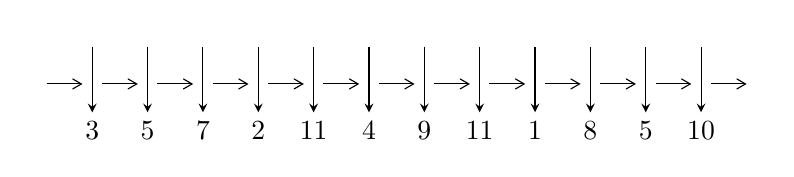
\begin{tikzpicture}[x=20pt, y=17pt]
	% nodes
	\node (C0) at (0, 0) {};
	\node (C1) at (1, 0) {};
	\node (C1U) at (1, +1) {};
	\node (C1D) at (1, -1) {3};

	\node (C2) at (2, 0) {};
	\node (C2U) at (2, +1) {};
	\node (C2D) at (2, -1) {5};

	\node (C3) at (3, 0) {};
	\node (C3U) at (3, +1) {};
	\node (C3D) at (3, -1) {7};

	\node (C4) at (4, 0) {};
	\node (C4U) at (4, +1) {};
	\node (C4D) at (4, -1) {2};

	\node (C5) at (5, 0) {};
	\node (C5U) at (5, +1) {};
	\node (C5D) at (5, -1) {11};

	\node (C6) at (6, 0) {};
	\node (C6U) at (6, +1) {};
	\node (C6D) at (6, -1) {4};

	\node (C7) at (7, 0) {};
	\node (C7U) at (7, +1) {};
	\node (C7D) at (7, -1) {9};

	\node (C8) at (8, 0) {};
	\node (C8U) at (8, +1) {};
	\node (C8D) at (8, -1) {11};

	\node (C9) at (9, 0) {};
	\node (C9U) at (9, +1) {};
	\node (C9D) at (9, -1) {1};

	\node (C10) at (10, 0) {};
	\node (C10U) at (10, +1) {};
	\node (C10D) at (10, -1) {8};

	\node (C11) at (11, 0) {};
	\node (C11U) at (11, +1) {};
	\node (C11D) at (11, -1) {5};

	\node (C12) at (12, 0) {};
	\node (C12U) at (12, +1) {};
	\node (C12D) at (12, -1) {10};
	\node (C13) at (13, 0) {};

	% arrows
	\draw[->,>={angle 60}]
	(C0) edge (C1) (C1) edge (C2) (C2) edge (C3) (C3) edge (C4) (C4) edge (C5) (C5) edge (C6) (C6) edge (C7) (C7) edge (C8) (C8) edge (C9) (C9) edge (C10) (C10) edge (C11) (C11) edge (C12) (C12) edge (C13) ;	\draw[->,>=stealth]
	(C1U) edge (C1D) (C2U) edge (C2D) (C3U) edge (C3D) (C4U) edge (C4D) (C5U) edge (C5D) (C6U) edge (C6D) (C7U) edge (C7D) (C8U) edge (C8D) (C9U) edge (C9D) (C10U) edge (C10D) (C11U) edge (C11D) (C12U) edge (C12D) ;
	\end{tikzpicture} \\
\hhline{~~} \\& 
\textbf{Solving Sequence} \\ \cline{2-2} 
 &
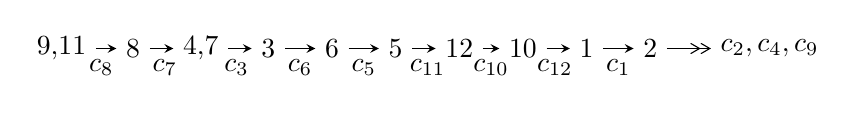
\begin{tikzpicture}[x=23pt, y=7pt]
	% node
	\node (A0) at (-1/8, 0) {9,11};
	\node (A1) at (1, 0) {8};
	\node (A2) at (33/16, 0) {4,7};
	\node (A3) at (25/8, 0) {3};
	\node (A4) at (33/8, 0) {6};
	\node (A5) at (41/8, 0) {5};
	\node (A6) at (49/8, 0) {12};
	\node (A7) at (57/8, 0) {10};
	\node (A8) at (65/8, 0) {1};
	\node (A9) at (73/8, 0) {2};
	\node (C1) at (1/2, -1) {$c_{8}$};
	\node (C2) at (3/2, -1) {$c_{7}$};
	\node (C3) at (21/8, -1) {$c_{3}$};
	\node (C4) at (29/8, -1) {$c_{6}$};
	\node (C5) at (37/8, -1) {$c_{5}$};
	\node (C6) at (45/8, -1) {$c_{11}$};
	\node (C7) at (53/8, -1) {$c_{10}$};
	\node (C8) at (61/8, -1) {$c_{12}$};
	\node (C9) at (69/8, -1) {$c_{1}$};
	\node (A10) at (11, 0) {$c_{2},c_{4},c_{9}$};

	% edge
	\draw[->,>=stealth]	
	(A0) edge (A1) (A1) edge (A2) (A2) edge (A3) (A3) edge (A4) (A4) edge (A5) (A5) edge (A6) (A6) edge (A7) (A7) edge (A8) (A8) edge (A9) ;
	\draw[->>,>={angle 60}]	
	(A9) edge (A10);
\end{tikzpicture} \\ 

\end{tabular} \\

\footnotetext{
The image of knot diagram is generated by the software ``\textbf{Draw programme}" developed by Andrew Bartholomew(\url{http://www.layer8.co.uk/maths/draw/index.htm\#Running-draw}), where we modified some parts for our purpose(\url{https://github.com/CATsTAILs/LinksPainter}).
}\phantom \\ \newline 
\centering \textbf{Ideals for irreducible components\footnotemark of $X_{\text{par}}$} 
 
\begin{align*}
I^u_{1}&=\langle 
2 u^{13}+5 u^{12}-2 u^{11}-16 u^{10}-10 u^9+16 u^8+28 u^7+10 u^6-19 u^5-25 u^4-7 u^3+6 u^2+2 b+5 u,\\
\phantom{I^u_{1}}&\phantom{= \langle  }- u^{13}-4 u^{12}-3 u^{11}+8 u^{10}+14 u^9-18 u^7-21 u^6-5 u^5+16 u^4+17 u^3+4 u^2+2 a-4 u-5,\\
\phantom{I^u_{1}}&\phantom{= \langle  }u^{14}+3 u^{13}-9 u^{11}-8 u^{10}+8 u^9+18 u^8+9 u^7-10 u^6-18 u^5-6 u^4+6 u^3+6 u^2+2 u-1\rangle \\
I^u_{2}&=\langle 
-1.17690\times10^{65} u^{57}-3.97295\times10^{65} u^{56}+\cdots+3.56133\times10^{64} b-4.96718\times10^{63},\\
\phantom{I^u_{2}}&\phantom{= \langle  }-6.29210\times10^{64} u^{57}-8.59795\times10^{64} u^{56}+\cdots+7.12266\times10^{64} a-4.18226\times10^{65},\;u^{58}+4 u^{57}+\cdots-5 u+1\rangle \\
I^u_{3}&=\langle 
u^2+b+u-1,\;a+u,\;u^3+u^2-1\rangle \\
I^u_{4}&=\langle 
4 u^2 a+6 a u+b+4 a+1,\;-2 u^2 a+a^2- a u-2 u^2+2 a- u+2,\;u^3+u^2-1\rangle \\
I^u_{5}&=\langle 
b- u-2,\;a+2 u+3,\;u^2+u-1\rangle \\
I^u_{6}&=\langle 
b-2 a+2,\;a^2- a-1,\;u-1\rangle \\
\\
\end{align*}
\raggedright * 6 irreducible components of $\dim_{\mathbb{C}}=0$, with total 85 representations.\\
\footnotetext{All coefficients of polynomials are rational numbers. But the coefficients are sometimes approximated in decimal forms when there is not enough margin.}
\newpage
\renewcommand{\arraystretch}{1}
\centering \section*{I. $I^u_{1}= \langle 2 u^{13}+5 u^{12}+\cdots+2 b+5 u,\;- u^{13}-4 u^{12}+\cdots+2 a-5,\;u^{14}+3 u^{13}+\cdots+2 u-1 \rangle$}
\flushleft \textbf{(i) Arc colorings}\\
\begin{tabular}{m{7pt} m{180pt} m{7pt} m{180pt} }
\flushright $a_{9}=$&$\begin{pmatrix}1\\0\end{pmatrix}$ \\
\flushright $a_{11}=$&$\begin{pmatrix}0\\u\end{pmatrix}$ \\
\flushright $a_{8}=$&$\begin{pmatrix}1\\- u^2\end{pmatrix}$ \\
\flushright $a_{4}=$&$\begin{pmatrix}\frac{1}{2} u^{13}+2 u^{12}+\cdots+2 u+\frac{5}{2}\\- u^{13}-\frac{5}{2} u^{12}+\cdots-3 u^2-\frac{5}{2} u\end{pmatrix}$ \\
\flushright $a_{7}=$&$\begin{pmatrix}- u^2+1\\- u^2\end{pmatrix}$ \\
\flushright $a_{3}=$&$\begin{pmatrix}\frac{1}{2} u^{13}+\frac{3}{2} u^{12}+\cdots+\frac{5}{2} u+2\\-\frac{1}{2} u^{13}-2 u^{12}+\cdots- u-\frac{1}{2}\end{pmatrix}$ \\
\flushright $a_{6}=$&$\begin{pmatrix}\frac{1}{2} u^{13}+\frac{3}{2} u^{12}+\cdots+\frac{3}{2} u+2\\-\frac{1}{2} u^{12}-\frac{3}{2} u^{11}+\cdots-\frac{1}{2} u-\frac{1}{2}\end{pmatrix}$ \\
\flushright $a_{5}=$&$\begin{pmatrix}\frac{1}{2} u^{13}+\frac{3}{2} u^{12}+\cdots+\frac{3}{2} u+2\\- u^{12}-\frac{5}{2} u^{11}+\cdots- u-\frac{1}{2}\end{pmatrix}$ \\
\flushright $a_{12}=$&$\begin{pmatrix}- u^{11}- u^{10}+3 u^9+4 u^8-3 u^7-6 u^6-2 u^5+3 u^4+5 u^3+u^2-2 u-1\\u^{13}+\frac{3}{2} u^{12}+\cdots+3 u^2+\frac{3}{2} u\end{pmatrix}$ \\
\flushright $a_{10}=$&$\begin{pmatrix}u\\- u^3+u\end{pmatrix}$ \\
\flushright $a_{1}=$&$\begin{pmatrix}\frac{1}{2} u^{13}+u^{12}+\cdots- u-\frac{3}{2}\\\frac{1}{2} u^{13}+u^{12}+\cdots+\frac{7}{2} u^2+u\end{pmatrix}$ \\
\flushright $a_{2}=$&$\begin{pmatrix}-\frac{1}{2} u^{13}-\frac{3}{2} u^{12}+\cdots-\frac{3}{2} u-\frac{3}{2}\\-\frac{1}{2} u^{13}-\frac{1}{2} u^{12}+\cdots+\frac{1}{2} u+\frac{1}{2}\end{pmatrix}$\\&\end{tabular}
\flushleft \textbf{(ii) Obstruction class $= -1$}\\~\\
\flushleft \textbf{(iii) Cusp Shapes $= 3 u^{13}+3 u^{12}-15 u^{11}-24 u^{10}+14 u^9+44 u^8+18 u^7-27 u^6-52 u^5-25 u^4+14 u^3+10 u^2+3 u-11$}\\~\\
\newpage\renewcommand{\arraystretch}{1}
\flushleft \textbf{(iv) u-Polynomials at the component}\newline \\
\begin{tabular}{m{50pt}|m{274pt}}
Crossings & \hspace{64pt}u-Polynomials at each crossing \\
\hline $$\begin{aligned}c_{1},c_{7}\end{aligned}$$&$\begin{aligned}
&u^{14}+9 u^{13}+\cdots+16 u+1
\end{aligned}$\\
\hline $$\begin{aligned}c_{2},c_{4},c_{8}\\c_{10}\end{aligned}$$&$\begin{aligned}
&u^{14}-3 u^{13}+\cdots-2 u-1
\end{aligned}$\\
\hline $$\begin{aligned}c_{3},c_{6},c_{9}\\c_{12}\end{aligned}$$&$\begin{aligned}
&u^{14}- u^{13}+\cdots-4 u-1
\end{aligned}$\\
\hline $$\begin{aligned}c_{5},c_{11}\end{aligned}$$&$\begin{aligned}
&u^{14}-7 u^{13}+\cdots-24 u+8
\end{aligned}$\\
\hline
\end{tabular}\\~\\
\newpage\renewcommand{\arraystretch}{1}
\flushleft \textbf{(v) Riley Polynomials at the component}\newline \\
\begin{tabular}{m{50pt}|m{274pt}}
Crossings & \hspace{64pt}Riley Polynomials at each crossing \\
\hline $$\begin{aligned}c_{1},c_{7}\end{aligned}$$&$\begin{aligned}
&y^{14}-5 y^{13}+\cdots-208 y+1
\end{aligned}$\\
\hline $$\begin{aligned}c_{2},c_{4},c_{8}\\c_{10}\end{aligned}$$&$\begin{aligned}
&y^{14}-9 y^{13}+\cdots-16 y+1
\end{aligned}$\\
\hline $$\begin{aligned}c_{3},c_{6},c_{9}\\c_{12}\end{aligned}$$&$\begin{aligned}
&y^{14}+3 y^{13}+\cdots-8 y+1
\end{aligned}$\\
\hline $$\begin{aligned}c_{5},c_{11}\end{aligned}$$&$\begin{aligned}
&y^{14}-7 y^{13}+\cdots+384 y+64
\end{aligned}$\\
\hline
\end{tabular}\\~\\
\newpage\flushleft \textbf{(vi) Complex Volumes and Cusp Shapes}
$$\begin{array}{c|c|c}  
\text{Solutions to }I^u_{1}& \I (\text{vol} + \sqrt{-1}CS) & \text{Cusp shape}\\
 \hline 
\begin{aligned}
u &= -0.242991 + 0.933745 I \\
a &= -0.20291 + 1.67953 I \\
b &= -0.821533 + 0.270883 I\end{aligned}
 & \phantom{-}1.33116 - 5.50874 I & -7.69545 + 3.70076 I \\ \hline\begin{aligned}
u &= -0.242991 - 0.933745 I \\
a &= -0.20291 - 1.67953 I \\
b &= -0.821533 - 0.270883 I\end{aligned}
 & \phantom{-}1.33116 + 5.50874 I & -7.69545 - 3.70076 I \\ \hline\begin{aligned}
u &= \phantom{-}0.951606 + 0.107631 I \\
a &= -0.80680 + 1.21543 I \\
b &= \phantom{-}3.80232 + 0.74412 I\end{aligned}
 & -2.88995 - 0.46660 I & -33.6526 - 15.6404 I \\ \hline\begin{aligned}
u &= \phantom{-}0.951606 - 0.107631 I \\
a &= -0.80680 - 1.21543 I \\
b &= \phantom{-}3.80232 - 0.74412 I\end{aligned}
 & -2.88995 + 0.46660 I & -33.6526 + 15.6404 I \\ \hline\begin{aligned}
u &= -0.389011 + 0.665748 I \\
a &= \phantom{-}0.507976 + 0.255319 I \\
b &= \phantom{-}0.587054 + 0.784524 I\end{aligned}
 & \phantom{-}3.75566 + 0.17244 I & -4.31674 - 1.33622 I \\ \hline\begin{aligned}
u &= -0.389011 - 0.665748 I \\
a &= \phantom{-}0.507976 - 0.255319 I \\
b &= \phantom{-}0.587054 - 0.784524 I\end{aligned}
 & \phantom{-}3.75566 - 0.17244 I & -4.31674 + 1.33622 I \\ \hline\begin{aligned}
u &= -1.217360 + 0.433191 I \\
a &= -0.051195 + 0.233560 I \\
b &= \phantom{-}0.695133 + 0.745943 I\end{aligned}
 & -1.53918 + 8.57795 I & -13.9694 - 8.6920 I \\ \hline\begin{aligned}
u &= -1.217360 - 0.433191 I \\
a &= -0.051195 - 0.233560 I \\
b &= \phantom{-}0.695133 - 0.745943 I\end{aligned}
 & -1.53918 - 8.57795 I & -13.9694 + 8.6920 I \\ \hline\begin{aligned}
u &= \phantom{-}1.208510 + 0.461890 I \\
a &= \phantom{-}1.195780 - 0.437447 I \\
b &= \phantom{-}1.55260 - 0.60463 I\end{aligned}
 & -7.24910 - 2.92807 I & -16.0849 + 1.6852 I \\ \hline\begin{aligned}
u &= \phantom{-}1.208510 - 0.461890 I \\
a &= \phantom{-}1.195780 + 0.437447 I \\
b &= \phantom{-}1.55260 + 0.60463 I\end{aligned}
 & -7.24910 + 2.92807 I & -16.0849 - 1.6852 I\\
 \hline 
 \end{array}$$\newpage$$\begin{array}{c|c|c}  
\text{Solutions to }I^u_{1}& \I (\text{vol} + \sqrt{-1}CS) & \text{Cusp shape}\\
 \hline 
\begin{aligned}
u &= -1.31782\phantom{ +0.000000I} \\
a &= \phantom{-}0.941660\phantom{ +0.000000I} \\
b &= \phantom{-}0.882448\phantom{ +0.000000I}\end{aligned}
 & -10.4546\phantom{ +0.000000I} & -24.6220\phantom{ +0.000000I} \\ \hline\begin{aligned}
u &= -1.28364 + 0.61767 I \\
a &= -1.46437 - 0.09958 I \\
b &= -2.38982 - 1.44096 I\end{aligned}
 & -4.9818 + 17.0516 I & -13.2441 - 9.4300 I \\ \hline\begin{aligned}
u &= -1.28364 - 0.61767 I \\
a &= -1.46437 + 0.09958 I \\
b &= -2.38982 + 1.44096 I\end{aligned}
 & -4.9818 - 17.0516 I & -13.2441 + 9.4300 I \\ \hline\begin{aligned}
u &= \phantom{-}0.263596\phantom{ +0.000000I} \\
a &= \phantom{-}2.70137\phantom{ +0.000000I} \\
b &= -0.733954\phantom{ +0.000000I}\end{aligned}
 & -0.942520\phantom{ +0.000000I} & -9.45120\phantom{ +0.000000I}\\
 \hline 
 \end{array}$$\newpage\newpage\renewcommand{\arraystretch}{1}
\centering \section*{II. $I^u_{2}= \langle -1.18\times10^{65} u^{57}-3.97\times10^{65} u^{56}+\cdots+3.56\times10^{64} b-4.97\times10^{63},\;-6.29\times10^{64} u^{57}-8.60\times10^{64} u^{56}+\cdots+7.12\times10^{64} a-4.18\times10^{65},\;u^{58}+4 u^{57}+\cdots-5 u+1 \rangle$}
\flushleft \textbf{(i) Arc colorings}\\
\begin{tabular}{m{7pt} m{180pt} m{7pt} m{180pt} }
\flushright $a_{9}=$&$\begin{pmatrix}1\\0\end{pmatrix}$ \\
\flushright $a_{11}=$&$\begin{pmatrix}0\\u\end{pmatrix}$ \\
\flushright $a_{8}=$&$\begin{pmatrix}1\\- u^2\end{pmatrix}$ \\
\flushright $a_{4}=$&$\begin{pmatrix}0.883391 u^{57}+1.20713 u^{56}+\cdots-9.91542 u+5.87176\\3.30467 u^{57}+11.1558 u^{56}+\cdots-6.41751 u+0.139475\end{pmatrix}$ \\
\flushright $a_{7}=$&$\begin{pmatrix}- u^2+1\\- u^2\end{pmatrix}$ \\
\flushright $a_{3}=$&$\begin{pmatrix}0.793575 u^{57}+0.365747 u^{56}+\cdots-3.89250 u+4.38523\\1.32573 u^{57}+4.64753 u^{56}+\cdots+4.91950 u-1.75010\end{pmatrix}$ \\
\flushright $a_{6}=$&$\begin{pmatrix}1.70888 u^{57}+4.42480 u^{56}+\cdots-6.68595 u+4.41639\\2.56867 u^{57}+8.73466 u^{56}+\cdots-12.4165 u+1.63075\end{pmatrix}$ \\
\flushright $a_{5}=$&$\begin{pmatrix}1.70888 u^{57}+4.42480 u^{56}+\cdots-6.68595 u+4.41639\\0.322307 u^{57}+1.39608 u^{56}+\cdots+1.34584 u-0.779945\end{pmatrix}$ \\
\flushright $a_{12}=$&$\begin{pmatrix}1.31808 u^{57}+3.67421 u^{56}+\cdots+1.92169 u-2.00892\\0.489553 u^{57}+1.26691 u^{56}+\cdots-0.411200 u+0.625023\end{pmatrix}$ \\
\flushright $a_{10}=$&$\begin{pmatrix}u\\- u^3+u\end{pmatrix}$ \\
\flushright $a_{1}=$&$\begin{pmatrix}2.12433 u^{57}+5.66107 u^{56}+\cdots+3.12772 u-2.10774\\-0.0988242 u^{57}-1.20154 u^{56}+\cdots+7.79161 u-0.711908\end{pmatrix}$ \\
\flushright $a_{2}=$&$\begin{pmatrix}-0.453494 u^{57}-0.227312 u^{56}+\cdots+6.41674 u-3.64552\\-2.66084 u^{57}-9.70894 u^{56}+\cdots+11.5745 u-1.08534\end{pmatrix}$\\&\end{tabular}
\flushleft \textbf{(ii) Obstruction class $= -1$}\\~\\
\flushleft \textbf{(iii) Cusp Shapes $= 8.86204 u^{57}+41.6548 u^{56}+\cdots+50.2522 u-23.8526$}\\~\\
\newpage\renewcommand{\arraystretch}{1}
\flushleft \textbf{(iv) u-Polynomials at the component}\newline \\
\begin{tabular}{m{50pt}|m{274pt}}
Crossings & \hspace{64pt}u-Polynomials at each crossing \\
\hline $$\begin{aligned}c_{1},c_{7}\end{aligned}$$&$\begin{aligned}
&u^{58}+32 u^{57}+\cdots+25 u+1
\end{aligned}$\\
\hline $$\begin{aligned}c_{2},c_{4},c_{8}\\c_{10}\end{aligned}$$&$\begin{aligned}
&u^{58}-4 u^{57}+\cdots+5 u+1
\end{aligned}$\\
\hline $$\begin{aligned}c_{3},c_{6},c_{9}\\c_{12}\end{aligned}$$&$\begin{aligned}
&u^{58}-4 u^{57}+\cdots+32 u-4
\end{aligned}$\\
\hline $$\begin{aligned}c_{5},c_{11}\end{aligned}$$&$\begin{aligned}
&(u^{29}+2 u^{28}+\cdots-28 u-8)^{2}
\end{aligned}$\\
\hline
\end{tabular}\\~\\
\newpage\renewcommand{\arraystretch}{1}
\flushleft \textbf{(v) Riley Polynomials at the component}\newline \\
\begin{tabular}{m{50pt}|m{274pt}}
Crossings & \hspace{64pt}Riley Polynomials at each crossing \\
\hline $$\begin{aligned}c_{1},c_{7}\end{aligned}$$&$\begin{aligned}
&y^{58}-8 y^{57}+\cdots+195 y+1
\end{aligned}$\\
\hline $$\begin{aligned}c_{2},c_{4},c_{8}\\c_{10}\end{aligned}$$&$\begin{aligned}
&y^{58}-32 y^{57}+\cdots-25 y+1
\end{aligned}$\\
\hline $$\begin{aligned}c_{3},c_{6},c_{9}\\c_{12}\end{aligned}$$&$\begin{aligned}
&y^{58}+18 y^{57}+\cdots-984 y+16
\end{aligned}$\\
\hline $$\begin{aligned}c_{5},c_{11}\end{aligned}$$&$\begin{aligned}
&(y^{29}-28 y^{28}+\cdots+2896 y-64)^{2}
\end{aligned}$\\
\hline
\end{tabular}\\~\\
\newpage\flushleft \textbf{(vi) Complex Volumes and Cusp Shapes}
$$\begin{array}{c|c|c}  
\text{Solutions to }I^u_{2}& \I (\text{vol} + \sqrt{-1}CS) & \text{Cusp shape}\\
 \hline 
\begin{aligned}
u &= \phantom{-}0.988988\phantom{ +0.000000I} \\
a &= -0.481132\phantom{ +0.000000I} \\
b &= -5.97136\phantom{ +0.000000I}\end{aligned}
 & -2.67255\phantom{ +0.000000I} & -211.680\phantom{ +0.000000I} \\ \hline\begin{aligned}
u &= -0.852515 + 0.455377 I \\
a &= \phantom{-}0.096402 + 0.221595 I \\
b &= \phantom{-}1.14950 + 1.39220 I\end{aligned}
 & \phantom{-}4.34822 + 5.30129 I & -10.14110 - 5.91971 I \\ \hline\begin{aligned}
u &= -0.852515 - 0.455377 I \\
a &= \phantom{-}0.096402 - 0.221595 I \\
b &= \phantom{-}1.14950 - 1.39220 I\end{aligned}
 & \phantom{-}4.34822 - 5.30129 I & -10.14110 + 5.91971 I \\ \hline\begin{aligned}
u &= -0.875378 + 0.395680 I \\
a &= -1.17395 - 1.12502 I \\
b &= -0.55207 - 1.63441 I\end{aligned}
 & -1.15248 + 2.97907 I & -9.53425 - 4.84429 I \\ \hline\begin{aligned}
u &= -0.875378 - 0.395680 I \\
a &= -1.17395 + 1.12502 I \\
b &= -0.55207 + 1.63441 I\end{aligned}
 & -1.15248 - 2.97907 I & -9.53425 + 4.84429 I \\ \hline\begin{aligned}
u &= \phantom{-}0.382222 + 0.979860 I \\
a &= \phantom{-}0.37822 + 1.49048 I \\
b &= \phantom{-}0.968996 + 0.458325 I\end{aligned}
 & -4.05295 + 3.42058 I & -12.00000 - 4.03802 I \\ \hline\begin{aligned}
u &= \phantom{-}0.382222 - 0.979860 I \\
a &= \phantom{-}0.37822 - 1.49048 I \\
b &= \phantom{-}0.968996 - 0.458325 I\end{aligned}
 & -4.05295 - 3.42058 I & -12.00000 + 4.03802 I \\ \hline\begin{aligned}
u &= -1.06017\phantom{ +0.000000I} \\
a &= \phantom{-}1.48801\phantom{ +0.000000I} \\
b &= \phantom{-}1.19467\phantom{ +0.000000I}\end{aligned}
 & -10.6310\phantom{ +0.000000I} & -48.5360\phantom{ +0.000000I} \\ \hline\begin{aligned}
u &= -0.216051 + 1.075610 I \\
a &= \phantom{-}0.49789 - 1.82352 I \\
b &= \phantom{-}0.930330 - 0.518578 I\end{aligned}
 & -1.66044 - 11.01250 I & -12.00000 + 0. I\phantom{ +0.000000I} \\ \hline\begin{aligned}
u &= -0.216051 - 1.075610 I \\
a &= \phantom{-}0.49789 + 1.82352 I \\
b &= \phantom{-}0.930330 + 0.518578 I\end{aligned}
 & -1.66044 + 11.01250 I & -12.00000 + 0. I\phantom{ +0.000000I}\\
 \hline 
 \end{array}$$\newpage$$\begin{array}{c|c|c}  
\text{Solutions to }I^u_{2}& \I (\text{vol} + \sqrt{-1}CS) & \text{Cusp shape}\\
 \hline 
\begin{aligned}
u &= \phantom{-}0.994844 + 0.502352 I \\
a &= -0.026325 - 0.357537 I \\
b &= -1.077780 - 0.102508 I\end{aligned}
 & -0.488787 + 0.370462 I & \phantom{-0.000000 } 0 \\ \hline\begin{aligned}
u &= \phantom{-}0.994844 - 0.502352 I \\
a &= -0.026325 + 0.357537 I \\
b &= -1.077780 + 0.102508 I\end{aligned}
 & -0.488787 - 0.370462 I & \phantom{-0.000000 } 0 \\ \hline\begin{aligned}
u &= -0.108845 + 0.869895 I \\
a &= \phantom{-}0.31064 + 1.79296 I \\
b &= \phantom{-}0.569231 + 0.371365 I\end{aligned}
 & -3.19564 - 4.35308 I & -12.04263 + 3.74313 I \\ \hline\begin{aligned}
u &= -0.108845 - 0.869895 I \\
a &= \phantom{-}0.31064 - 1.79296 I \\
b &= \phantom{-}0.569231 - 0.371365 I\end{aligned}
 & -3.19564 + 4.35308 I & -12.04263 - 3.74313 I \\ \hline\begin{aligned}
u &= -1.006590 + 0.537430 I \\
a &= \phantom{-}0.312868 + 0.518025 I \\
b &= -0.632775 - 0.100970 I\end{aligned}
 & \phantom{-}2.03816 + 4.43643 I & \phantom{-0.000000 } 0 \\ \hline\begin{aligned}
u &= -1.006590 - 0.537430 I \\
a &= \phantom{-}0.312868 - 0.518025 I \\
b &= -0.632775 + 0.100970 I\end{aligned}
 & \phantom{-}2.03816 - 4.43643 I & \phantom{-0.000000 } 0 \\ \hline\begin{aligned}
u &= -0.873306 + 0.762690 I \\
a &= \phantom{-}2.26083 + 2.71765 I \\
b &= \phantom{-}0.21388 + 2.77675 I\end{aligned}
 & \phantom{-}1.81502 + 2.87998 I & \phantom{-0.000000 } 0 \\ \hline\begin{aligned}
u &= -0.873306 - 0.762690 I \\
a &= \phantom{-}2.26083 - 2.71765 I \\
b &= \phantom{-}0.21388 - 2.77675 I\end{aligned}
 & \phantom{-}1.81502 - 2.87998 I & \phantom{-0.000000 } 0 \\ \hline\begin{aligned}
u &= \phantom{-}0.836851 + 0.036106 I \\
a &= \phantom{-}0.0838767 - 0.0224097 I \\
b &= \phantom{-}0.00910 - 4.38592 I\end{aligned}
 & \phantom{-}1.81502 - 2.87998 I & -58.6220 + 17.5185 I \\ \hline\begin{aligned}
u &= \phantom{-}0.836851 - 0.036106 I \\
a &= \phantom{-}0.0838767 + 0.0224097 I \\
b &= \phantom{-}0.00910 + 4.38592 I\end{aligned}
 & \phantom{-}1.81502 + 2.87998 I & -58.6220 - 17.5185 I\\
 \hline 
 \end{array}$$\newpage$$\begin{array}{c|c|c}  
\text{Solutions to }I^u_{2}& \I (\text{vol} + \sqrt{-1}CS) & \text{Cusp shape}\\
 \hline 
\begin{aligned}
u &= -0.654785 + 0.491061 I \\
a &= \phantom{-}0.267178 + 0.146980 I \\
b &= -0.936070 - 0.955868 I\end{aligned}
 & \phantom{-}4.90257 - 1.34329 I & -7.80264 + 1.36225 I \\ \hline\begin{aligned}
u &= -0.654785 - 0.491061 I \\
a &= \phantom{-}0.267178 - 0.146980 I \\
b &= -0.936070 + 0.955868 I\end{aligned}
 & \phantom{-}4.90257 + 1.34329 I & -7.80264 - 1.36225 I \\ \hline\begin{aligned}
u &= -1.141310 + 0.406924 I \\
a &= -1.042680 - 0.445981 I \\
b &= -1.124050 - 0.134041 I\end{aligned}
 & -4.05295 + 3.42058 I & \phantom{-0.000000 } 0 \\ \hline\begin{aligned}
u &= -1.141310 - 0.406924 I \\
a &= -1.042680 + 0.445981 I \\
b &= -1.124050 + 0.134041 I\end{aligned}
 & -4.05295 - 3.42058 I & \phantom{-0.000000 } 0 \\ \hline\begin{aligned}
u &= -0.787150 + 0.924733 I \\
a &= \phantom{-}1.205180 - 0.532327 I \\
b &= \phantom{-}1.38107 + 0.43654 I\end{aligned}
 & \phantom{-}4.90257 + 1.34329 I & \phantom{-0.000000 } 0 \\ \hline\begin{aligned}
u &= -0.787150 - 0.924733 I \\
a &= \phantom{-}1.205180 + 0.532327 I \\
b &= \phantom{-}1.38107 - 0.43654 I\end{aligned}
 & \phantom{-}4.90257 - 1.34329 I & \phantom{-0.000000 } 0 \\ \hline\begin{aligned}
u &= \phantom{-}0.000304 + 0.780908 I \\
a &= -0.24339 - 2.24468 I \\
b &= \phantom{-}0.267868 - 0.277636 I\end{aligned}
 & -3.74876 - 1.54341 I & -12.07483 + 3.03548 I \\ \hline\begin{aligned}
u &= \phantom{-}0.000304 - 0.780908 I \\
a &= -0.24339 + 2.24468 I \\
b &= \phantom{-}0.267868 + 0.277636 I\end{aligned}
 & -3.74876 + 1.54341 I & -12.07483 - 3.03548 I \\ \hline\begin{aligned}
u &= \phantom{-}1.120680 + 0.529353 I \\
a &= \phantom{-}1.175230 - 0.118199 I \\
b &= \phantom{-}1.86181 - 1.77127 I\end{aligned}
 & -3.19564 - 4.35308 I & \phantom{-0.000000 } 0 \\ \hline\begin{aligned}
u &= \phantom{-}1.120680 - 0.529353 I \\
a &= \phantom{-}1.175230 + 0.118199 I \\
b &= \phantom{-}1.86181 + 1.77127 I\end{aligned}
 & -3.19564 + 4.35308 I & \phantom{-0.000000 } 0\\
 \hline 
 \end{array}$$\newpage$$\begin{array}{c|c|c}  
\text{Solutions to }I^u_{2}& \I (\text{vol} + \sqrt{-1}CS) & \text{Cusp shape}\\
 \hline 
\begin{aligned}
u &= -0.665448 + 0.320577 I \\
a &= -1.75785 - 0.27970 I \\
b &= -0.427413 - 0.048282 I\end{aligned}
 & -0.488787 + 0.370462 I & -8.36692 - 2.50640 I \\ \hline\begin{aligned}
u &= -0.665448 - 0.320577 I \\
a &= -1.75785 + 0.27970 I \\
b &= -0.427413 + 0.048282 I\end{aligned}
 & -0.488787 - 0.370462 I & -8.36692 + 2.50640 I \\ \hline\begin{aligned}
u &= -1.209970 + 0.458074 I \\
a &= -1.109810 - 0.614505 I \\
b &= -2.00916 - 2.00839 I\end{aligned}
 & -7.27243 + 6.00653 I & \phantom{-0.000000 } 0 \\ \hline\begin{aligned}
u &= -1.209970 - 0.458074 I \\
a &= -1.109810 + 0.614505 I \\
b &= -2.00916 + 2.00839 I\end{aligned}
 & -7.27243 - 6.00653 I & \phantom{-0.000000 } 0 \\ \hline\begin{aligned}
u &= \phantom{-}1.264110 + 0.277934 I \\
a &= -0.094671 - 0.217784 I \\
b &= \phantom{-}0.589009 + 0.036358 I\end{aligned}
 & -1.15248 - 2.97907 I & \phantom{-0.000000 } 0 \\ \hline\begin{aligned}
u &= \phantom{-}1.264110 - 0.277934 I \\
a &= -0.094671 + 0.217784 I \\
b &= \phantom{-}0.589009 - 0.036358 I\end{aligned}
 & -1.15248 + 2.97907 I & \phantom{-0.000000 } 0 \\ \hline\begin{aligned}
u &= \phantom{-}1.278760 + 0.279605 I \\
a &= -0.874635 + 0.506037 I \\
b &= -1.179270 + 0.382768 I\end{aligned}
 & -3.74876 + 1.54341 I & \phantom{-0.000000 } 0 \\ \hline\begin{aligned}
u &= \phantom{-}1.278760 - 0.279605 I \\
a &= -0.874635 - 0.506037 I \\
b &= -1.179270 - 0.382768 I\end{aligned}
 & -3.74876 - 1.54341 I & \phantom{-0.000000 } 0 \\ \hline\begin{aligned}
u &= \phantom{-}0.689587\phantom{ +0.000000I} \\
a &= \phantom{-}6.16946\phantom{ +0.000000I} \\
b &= -5.31315\phantom{ +0.000000I}\end{aligned}
 & -2.67255\phantom{ +0.000000I} & -211.680\phantom{ +0.000000I} \\ \hline\begin{aligned}
u &= \phantom{-}1.251940 + 0.396137 I \\
a &= -1.204600 + 0.452476 I \\
b &= -2.28308 + 2.02996 I\end{aligned}
 & -7.39364\phantom{ +0.000000I} & \phantom{-0.000000 } 0\\
 \hline 
 \end{array}$$\newpage$$\begin{array}{c|c|c}  
\text{Solutions to }I^u_{2}& \I (\text{vol} + \sqrt{-1}CS) & \text{Cusp shape}\\
 \hline 
\begin{aligned}
u &= \phantom{-}1.251940 - 0.396137 I \\
a &= -1.204600 - 0.452476 I \\
b &= -2.28308 - 2.02996 I\end{aligned}
 & -7.39364\phantom{ +0.000000I} & \phantom{-0.000000 } 0 \\ \hline\begin{aligned}
u &= \phantom{-}0.027420 + 0.672723 I \\
a &= \phantom{-}0.367381 + 0.017368 I \\
b &= -0.180737 - 0.719838 I\end{aligned}
 & \phantom{-}2.03816 - 4.43643 I & -7.12586 + 5.70665 I \\ \hline\begin{aligned}
u &= \phantom{-}0.027420 - 0.672723 I \\
a &= \phantom{-}0.367381 - 0.017368 I \\
b &= -0.180737 + 0.719838 I\end{aligned}
 & \phantom{-}2.03816 + 4.43643 I & -7.12586 - 5.70665 I \\ \hline\begin{aligned}
u &= -1.227590 + 0.512752 I \\
a &= \phantom{-}1.029830 + 0.433526 I \\
b &= \phantom{-}1.235900 + 0.213650 I\end{aligned}
 & -6.56035 + 9.36152 I & \phantom{-0.000000 } 0 \\ \hline\begin{aligned}
u &= -1.227590 - 0.512752 I \\
a &= \phantom{-}1.029830 - 0.433526 I \\
b &= \phantom{-}1.235900 - 0.213650 I\end{aligned}
 & -6.56035 - 9.36152 I & \phantom{-0.000000 } 0 \\ \hline\begin{aligned}
u &= -0.984255 + 0.909262 I \\
a &= -1.077810 + 0.708898 I \\
b &= -1.52408 - 0.24363 I\end{aligned}
 & \phantom{-}4.34822 + 5.30129 I & \phantom{-0.000000 } 0 \\ \hline\begin{aligned}
u &= -0.984255 - 0.909262 I \\
a &= -1.077810 - 0.708898 I \\
b &= -1.52408 + 0.24363 I\end{aligned}
 & \phantom{-}4.34822 - 5.30129 I & \phantom{-0.000000 } 0 \\ \hline\begin{aligned}
u &= -1.220950 + 0.580073 I \\
a &= \phantom{-}1.236460 + 0.202005 I \\
b &= \phantom{-}2.15316 + 1.56889 I\end{aligned}
 & -1.66044 + 11.01250 I & \phantom{-0.000000 } 0 \\ \hline\begin{aligned}
u &= -1.220950 - 0.580073 I \\
a &= \phantom{-}1.236460 - 0.202005 I \\
b &= \phantom{-}2.15316 - 1.56889 I\end{aligned}
 & -1.66044 - 11.01250 I & \phantom{-0.000000 } 0 \\ \hline\begin{aligned}
u &= \phantom{-}1.196500 + 0.654445 I \\
a &= -1.393060 + 0.026552 I \\
b &= -2.02586 + 1.44130 I\end{aligned}
 & -6.56035 - 9.36152 I & \phantom{-0.000000 } 0\\
 \hline 
 \end{array}$$\newpage$$\begin{array}{c|c|c}  
\text{Solutions to }I^u_{2}& \I (\text{vol} + \sqrt{-1}CS) & \text{Cusp shape}\\
 \hline 
\begin{aligned}
u &= \phantom{-}1.196500 - 0.654445 I \\
a &= -1.393060 - 0.026552 I \\
b &= -2.02586 - 1.44130 I\end{aligned}
 & -6.56035 + 9.36152 I & \phantom{-0.000000 } 0 \\ \hline\begin{aligned}
u &= \phantom{-}1.44823 + 0.32172 I \\
a &= \phantom{-}0.885882 - 0.795017 I \\
b &= \phantom{-}0.993193 - 0.775693 I\end{aligned}
 & -7.27243 + 6.00653 I & \phantom{-0.000000 } 0 \\ \hline\begin{aligned}
u &= \phantom{-}1.44823 - 0.32172 I \\
a &= \phantom{-}0.885882 + 0.795017 I \\
b &= \phantom{-}0.993193 + 0.775693 I\end{aligned}
 & -7.27243 - 6.00653 I & \phantom{-0.000000 } 0 \\ \hline\begin{aligned}
u &= -1.57371\phantom{ +0.000000I} \\
a &= \phantom{-}0.372440\phantom{ +0.000000I} \\
b &= \phantom{-}0.379153\phantom{ +0.000000I}\end{aligned}
 & -10.6310\phantom{ +0.000000I} & \phantom{-0.000000 } 0 \\ \hline\begin{aligned}
u &= \phantom{-}0.242019 + 0.246574 I \\
a &= \phantom{-}1.39952 - 1.87926 I \\
b &= -0.768573 - 0.066926 I\end{aligned}
 & -0.942618\phantom{ +0.000000I} & -9.31087 + 0. I\phantom{ +0.000000I} \\ \hline\begin{aligned}
u &= \phantom{-}0.242019 - 0.246574 I \\
a &= \phantom{-}1.39952 + 1.87926 I \\
b &= -0.768573 + 0.066926 I\end{aligned}
 & -0.942618\phantom{ +0.000000I} & -9.31087 + 0. I\phantom{ +0.000000I} \\ \hline\begin{aligned}
u &= \phantom{-}0.257910 + 0.127141 I \\
a &= \phantom{-}2.21702 - 1.31285 I \\
b &= -0.746774 - 0.028572 I\end{aligned}
 & -0.942376\phantom{ +0.000000I} & -9.38299 + 0. I\phantom{ +0.000000I} \\ \hline\begin{aligned}
u &= \phantom{-}0.257910 - 0.127141 I \\
a &= \phantom{-}2.21702 + 1.31285 I \\
b &= -0.746774 + 0.028572 I\end{aligned}
 & -0.942376\phantom{ +0.000000I} & -9.38299 + 0. I\phantom{ +0.000000I}\\
 \hline 
 \end{array}$$\newpage\newpage\renewcommand{\arraystretch}{1}
\centering \section*{III. $I^u_{3}= \langle u^2+b+u-1,\;a+u,\;u^3+u^2-1 \rangle$}
\flushleft \textbf{(i) Arc colorings}\\
\begin{tabular}{m{7pt} m{180pt} m{7pt} m{180pt} }
\flushright $a_{9}=$&$\begin{pmatrix}1\\0\end{pmatrix}$ \\
\flushright $a_{11}=$&$\begin{pmatrix}0\\u\end{pmatrix}$ \\
\flushright $a_{8}=$&$\begin{pmatrix}1\\- u^2\end{pmatrix}$ \\
\flushright $a_{4}=$&$\begin{pmatrix}- u\\- u^2- u+1\end{pmatrix}$ \\
\flushright $a_{7}=$&$\begin{pmatrix}- u^2+1\\- u^2\end{pmatrix}$ \\
\flushright $a_{3}=$&$\begin{pmatrix}-1\\0\end{pmatrix}$ \\
\flushright $a_{6}=$&$\begin{pmatrix}0\\- u\end{pmatrix}$ \\
\flushright $a_{5}=$&$\begin{pmatrix}0\\- u\end{pmatrix}$ \\
\flushright $a_{12}=$&$\begin{pmatrix}0\\u\end{pmatrix}$ \\
\flushright $a_{10}=$&$\begin{pmatrix}u\\u^2+u-1\end{pmatrix}$ \\
\flushright $a_{1}=$&$\begin{pmatrix}u^2-1\\u^2\end{pmatrix}$ \\
\flushright $a_{2}=$&$\begin{pmatrix}-1\\u^2\end{pmatrix}$\\&\end{tabular}
\flushleft \textbf{(ii) Obstruction class $= 1$}\\~\\
\flushleft \textbf{(iii) Cusp Shapes $= -8 u-12$}\\~\\
\newpage\renewcommand{\arraystretch}{1}
\flushleft \textbf{(iv) u-Polynomials at the component}\newline \\
\begin{tabular}{m{50pt}|m{274pt}}
Crossings & \hspace{64pt}u-Polynomials at each crossing \\
\hline $$\begin{aligned}c_{1},c_{3},c_{7}\\c_{9}\end{aligned}$$&$\begin{aligned}
&u^3- u^2+2 u-1
\end{aligned}$\\
\hline $$\begin{aligned}c_{2},c_{8}\end{aligned}$$&$\begin{aligned}
&u^3+u^2-1
\end{aligned}$\\
\hline $$\begin{aligned}c_{4},c_{10}\end{aligned}$$&$\begin{aligned}
&u^3- u^2+1
\end{aligned}$\\
\hline $$\begin{aligned}c_{5},c_{11}\end{aligned}$$&$\begin{aligned}
&u^3
\end{aligned}$\\
\hline $$\begin{aligned}c_{6},c_{12}\end{aligned}$$&$\begin{aligned}
&u^3+u^2+2 u+1
\end{aligned}$\\
\hline
\end{tabular}\\~\\
\newpage\renewcommand{\arraystretch}{1}
\flushleft \textbf{(v) Riley Polynomials at the component}\newline \\
\begin{tabular}{m{50pt}|m{274pt}}
Crossings & \hspace{64pt}Riley Polynomials at each crossing \\
\hline $$\begin{aligned}c_{1},c_{3},c_{6}\\c_{7},c_{9},c_{12}\end{aligned}$$&$\begin{aligned}
&y^3+3 y^2+2 y-1
\end{aligned}$\\
\hline $$\begin{aligned}c_{2},c_{4},c_{8}\\c_{10}\end{aligned}$$&$\begin{aligned}
&y^3- y^2+2 y-1
\end{aligned}$\\
\hline $$\begin{aligned}c_{5},c_{11}\end{aligned}$$&$\begin{aligned}
&y^3
\end{aligned}$\\
\hline
\end{tabular}\\~\\
\newpage\flushleft \textbf{(vi) Complex Volumes and Cusp Shapes}
$$\begin{array}{c|c|c}  
\text{Solutions to }I^u_{3}& \I (\text{vol} + \sqrt{-1}CS) & \text{Cusp shape}\\
 \hline 
\begin{aligned}
u &= -0.877439 + 0.744862 I \\
a &= \phantom{-}0.877439 - 0.744862 I \\
b &= \phantom{-}1.66236 + 0.56228 I\end{aligned}
 & \phantom{-}6.04826 + 5.65624 I & -4.98049 - 5.95889 I \\ \hline\begin{aligned}
u &= -0.877439 - 0.744862 I \\
a &= \phantom{-}0.877439 + 0.744862 I \\
b &= \phantom{-}1.66236 - 0.56228 I\end{aligned}
 & \phantom{-}6.04826 - 5.65624 I & -4.98049 + 5.95889 I \\ \hline\begin{aligned}
u &= \phantom{-}0.754878\phantom{ +0.000000I} \\
a &= -0.754878\phantom{ +0.000000I} \\
b &= -0.324718\phantom{ +0.000000I}\end{aligned}
 & -2.22691\phantom{ +0.000000I} & -18.0390\phantom{ +0.000000I}\\
 \hline 
 \end{array}$$\newpage\newpage\renewcommand{\arraystretch}{1}
\centering \section*{IV. $I^u_{4}= \langle 4 u^2 a+6 a u+b+4 a+1,\;-2 u^2 a+a^2- a u-2 u^2+2 a- u+2,\;u^3+u^2-1 \rangle$}
\flushleft \textbf{(i) Arc colorings}\\
\begin{tabular}{m{7pt} m{180pt} m{7pt} m{180pt} }
\flushright $a_{9}=$&$\begin{pmatrix}1\\0\end{pmatrix}$ \\
\flushright $a_{11}=$&$\begin{pmatrix}0\\u\end{pmatrix}$ \\
\flushright $a_{8}=$&$\begin{pmatrix}1\\- u^2\end{pmatrix}$ \\
\flushright $a_{4}=$&$\begin{pmatrix}a\\-4 u^2 a-6 a u-4 a-1\end{pmatrix}$ \\
\flushright $a_{7}=$&$\begin{pmatrix}- u^2+1\\- u^2\end{pmatrix}$ \\
\flushright $a_{3}=$&$\begin{pmatrix}- a u+u^2- u\\-3 u^2 a-5 a u-3 a- u\end{pmatrix}$ \\
\flushright $a_{6}=$&$\begin{pmatrix}0\\- u^2 a-2 a u+2 u^2-2 a+2 u+1\end{pmatrix}$ \\
\flushright $a_{5}=$&$\begin{pmatrix}0\\- u^2 a-2 a u+2 u^2-2 a+2 u+1\end{pmatrix}$ \\
\flushright $a_{12}=$&$\begin{pmatrix}0\\u\end{pmatrix}$ \\
\flushright $a_{10}=$&$\begin{pmatrix}u\\u^2+u-1\end{pmatrix}$ \\
\flushright $a_{1}=$&$\begin{pmatrix}u^2-1\\u^2\end{pmatrix}$ \\
\flushright $a_{2}=$&$\begin{pmatrix}- a u+u^2- u\\- u^2 a-2 a u+2 u^2- a+u+2\end{pmatrix}$\\&\end{tabular}
\flushleft \textbf{(ii) Obstruction class $= 1$}\\~\\
\flushleft \textbf{(iii) Cusp Shapes $= -16 u^2 a-21 a u-21 a+11 u-1$}\\~\\
\newpage\renewcommand{\arraystretch}{1}
\flushleft \textbf{(iv) u-Polynomials at the component}\newline \\
\begin{tabular}{m{50pt}|m{274pt}}
Crossings & \hspace{64pt}u-Polynomials at each crossing \\
\hline $$\begin{aligned}c_{1},c_{3},c_{7}\\c_{9}\end{aligned}$$&$\begin{aligned}
&(u^3- u^2+2 u-1)^2
\end{aligned}$\\
\hline $$\begin{aligned}c_{2},c_{8}\end{aligned}$$&$\begin{aligned}
&(u^3+u^2-1)^2
\end{aligned}$\\
\hline $$\begin{aligned}c_{4},c_{10}\end{aligned}$$&$\begin{aligned}
&(u^3- u^2+1)^2
\end{aligned}$\\
\hline $$\begin{aligned}c_{5},c_{11}\end{aligned}$$&$\begin{aligned}
&u^6
\end{aligned}$\\
\hline $$\begin{aligned}c_{6},c_{12}\end{aligned}$$&$\begin{aligned}
&(u^3+u^2+2 u+1)^2
\end{aligned}$\\
\hline
\end{tabular}\\~\\
\newpage\renewcommand{\arraystretch}{1}
\flushleft \textbf{(v) Riley Polynomials at the component}\newline \\
\begin{tabular}{m{50pt}|m{274pt}}
Crossings & \hspace{64pt}Riley Polynomials at each crossing \\
\hline $$\begin{aligned}c_{1},c_{3},c_{6}\\c_{7},c_{9},c_{12}\end{aligned}$$&$\begin{aligned}
&(y^3+3 y^2+2 y-1)^2
\end{aligned}$\\
\hline $$\begin{aligned}c_{2},c_{4},c_{8}\\c_{10}\end{aligned}$$&$\begin{aligned}
&(y^3- y^2+2 y-1)^2
\end{aligned}$\\
\hline $$\begin{aligned}c_{5},c_{11}\end{aligned}$$&$\begin{aligned}
&y^6
\end{aligned}$\\
\hline
\end{tabular}\\~\\
\newpage\flushleft \textbf{(vi) Complex Volumes and Cusp Shapes}
$$\begin{array}{c|c|c}  
\text{Solutions to }I^u_{4}& \I (\text{vol} + \sqrt{-1}CS) & \text{Cusp shape}\\
 \hline 
\begin{aligned}
u &= -0.877439 + 0.744862 I \\
a &= -1.069840 + 0.424452 I \\
b &= -1.75488 - 0.64082 I\end{aligned}
 & \phantom{-}6.04826\phantom{ +0.000000I} & -6.45445 + 0. I\phantom{ +0.000000I} \\ \hline\begin{aligned}
u &= -0.877439 + 0.744862 I \\
a &= -1.37744 - 2.29387 I \\
b &= \phantom{-}0.18504 - 1.97346 I\end{aligned}
 & \phantom{-}1.91067 + 2.82812 I & \phantom{-}9.7272 + 14.7292 I \\ \hline\begin{aligned}
u &= -0.877439 - 0.744862 I \\
a &= -1.069840 - 0.424452 I \\
b &= -1.75488 + 0.64082 I\end{aligned}
 & \phantom{-}6.04826\phantom{ +0.000000I} & -6.45445 + 0. I\phantom{ +0.000000I} \\ \hline\begin{aligned}
u &= -0.877439 - 0.744862 I \\
a &= -1.37744 + 2.29387 I \\
b &= \phantom{-}0.18504 + 1.97346 I\end{aligned}
 & \phantom{-}1.91067 - 2.82812 I & \phantom{-}9.7272 - 14.7292 I \\ \hline\begin{aligned}
u &= \phantom{-}0.754878\phantom{ +0.000000I} \\
a &= -0.052721 + 0.320410 I \\
b &= -0.43016 - 3.46319 I\end{aligned}
 & \phantom{-}1.91067 - 2.82812 I & \phantom{-}9.7272 - 14.7292 I \\ \hline\begin{aligned}
u &= \phantom{-}0.754878\phantom{ +0.000000I} \\
a &= -0.052721 - 0.320410 I \\
b &= -0.43016 + 3.46319 I\end{aligned}
 & \phantom{-}1.91067 + 2.82812 I & \phantom{-}9.7272 + 14.7292 I\\
 \hline 
 \end{array}$$\newpage\newpage\renewcommand{\arraystretch}{1}
\centering \section*{V. $I^u_{5}= \langle b- u-2,\;a+2 u+3,\;u^2+u-1 \rangle$}
\flushleft \textbf{(i) Arc colorings}\\
\begin{tabular}{m{7pt} m{180pt} m{7pt} m{180pt} }
\flushright $a_{9}=$&$\begin{pmatrix}1\\0\end{pmatrix}$ \\
\flushright $a_{11}=$&$\begin{pmatrix}0\\u\end{pmatrix}$ \\
\flushright $a_{8}=$&$\begin{pmatrix}1\\u-1\end{pmatrix}$ \\
\flushright $a_{4}=$&$\begin{pmatrix}-2 u-3\\u+2\end{pmatrix}$ \\
\flushright $a_{7}=$&$\begin{pmatrix}u\\u-1\end{pmatrix}$ \\
\flushright $a_{3}=$&$\begin{pmatrix}-2 u-3\\u+2\end{pmatrix}$ \\
\flushright $a_{6}=$&$\begin{pmatrix}u\\u-1\end{pmatrix}$ \\
\flushright $a_{5}=$&$\begin{pmatrix}u\\- u\end{pmatrix}$ \\
\flushright $a_{12}=$&$\begin{pmatrix}-2 u+1\\3 u-1\end{pmatrix}$ \\
\flushright $a_{10}=$&$\begin{pmatrix}u\\- u+1\end{pmatrix}$ \\
\flushright $a_{1}=$&$\begin{pmatrix}- u\\u\end{pmatrix}$ \\
\flushright $a_{2}=$&$\begin{pmatrix}-3 u-3\\2 u+2\end{pmatrix}$\\&\end{tabular}
\flushleft \textbf{(ii) Obstruction class $= 1$}\\~\\
\flushleft \textbf{(iii) Cusp Shapes $= 29$}\\~\\
\newpage\renewcommand{\arraystretch}{1}
\flushleft \textbf{(iv) u-Polynomials at the component}\newline \\
\begin{tabular}{m{50pt}|m{274pt}}
Crossings & \hspace{64pt}u-Polynomials at each crossing \\
\hline $$\begin{aligned}c_{1},c_{2}\end{aligned}$$&$\begin{aligned}
&(u-1)^2
\end{aligned}$\\
\hline $$\begin{aligned}c_{3},c_{6}\end{aligned}$$&$\begin{aligned}
&u^2
\end{aligned}$\\
\hline $$\begin{aligned}c_{4}\end{aligned}$$&$\begin{aligned}
&(u+1)^2
\end{aligned}$\\
\hline $$\begin{aligned}c_{5},c_{7}\end{aligned}$$&$\begin{aligned}
&u^2-3 u+1
\end{aligned}$\\
\hline $$\begin{aligned}c_{8},c_{9}\end{aligned}$$&$\begin{aligned}
&u^2+u-1
\end{aligned}$\\
\hline $$\begin{aligned}c_{10},c_{12}\end{aligned}$$&$\begin{aligned}
&u^2- u-1
\end{aligned}$\\
\hline $$\begin{aligned}c_{11}\end{aligned}$$&$\begin{aligned}
&u^2+3 u+1
\end{aligned}$\\
\hline
\end{tabular}\\~\\
\newpage\renewcommand{\arraystretch}{1}
\flushleft \textbf{(v) Riley Polynomials at the component}\newline \\
\begin{tabular}{m{50pt}|m{274pt}}
Crossings & \hspace{64pt}Riley Polynomials at each crossing \\
\hline $$\begin{aligned}c_{1},c_{2},c_{4}\end{aligned}$$&$\begin{aligned}
&(y-1)^2
\end{aligned}$\\
\hline $$\begin{aligned}c_{3},c_{6}\end{aligned}$$&$\begin{aligned}
&y^2
\end{aligned}$\\
\hline $$\begin{aligned}c_{5},c_{7},c_{11}\end{aligned}$$&$\begin{aligned}
&y^2-7 y+1
\end{aligned}$\\
\hline $$\begin{aligned}c_{8},c_{9},c_{10}\\c_{12}\end{aligned}$$&$\begin{aligned}
&y^2-3 y+1
\end{aligned}$\\
\hline
\end{tabular}\\~\\
\newpage\flushleft \textbf{(vi) Complex Volumes and Cusp Shapes}
$$\begin{array}{c|c|c}  
\text{Solutions to }I^u_{5}& \I (\text{vol} + \sqrt{-1}CS) & \text{Cusp shape}\\
 \hline 
\begin{aligned}
u &= \phantom{-}0.618034\phantom{ +0.000000I} \\
a &= -4.23607\phantom{ +0.000000I} \\
b &= \phantom{-}2.61803\phantom{ +0.000000I}\end{aligned}
 & -2.63189\phantom{ +0.000000I} & \phantom{-}29.0000\phantom{ +0.000000I} \\ \hline\begin{aligned}
u &= -1.61803\phantom{ +0.000000I} \\
a &= \phantom{-}0.236068\phantom{ +0.000000I} \\
b &= \phantom{-}0.381966\phantom{ +0.000000I}\end{aligned}
 & -10.5276\phantom{ +0.000000I} & \phantom{-}29.0000\phantom{ +0.000000I}\\
 \hline 
 \end{array}$$\newpage\newpage\renewcommand{\arraystretch}{1}
\centering \section*{VI. $I^u_{6}= \langle b-2 a+2,\;a^2- a-1,\;u-1 \rangle$}
\flushleft \textbf{(i) Arc colorings}\\
\begin{tabular}{m{7pt} m{180pt} m{7pt} m{180pt} }
\flushright $a_{9}=$&$\begin{pmatrix}1\\0\end{pmatrix}$ \\
\flushright $a_{11}=$&$\begin{pmatrix}0\\1\end{pmatrix}$ \\
\flushright $a_{8}=$&$\begin{pmatrix}1\\-1\end{pmatrix}$ \\
\flushright $a_{4}=$&$\begin{pmatrix}a\\2 a-2\end{pmatrix}$ \\
\flushright $a_{7}=$&$\begin{pmatrix}0\\-1\end{pmatrix}$ \\
\flushright $a_{3}=$&$\begin{pmatrix}a\\a-2\end{pmatrix}$ \\
\flushright $a_{6}=$&$\begin{pmatrix}- a-1\\-3\end{pmatrix}$ \\
\flushright $a_{5}=$&$\begin{pmatrix}- a-1\\a-2\end{pmatrix}$ \\
\flushright $a_{12}=$&$\begin{pmatrix}-3 a-2\\0\end{pmatrix}$ \\
\flushright $a_{10}=$&$\begin{pmatrix}1\\0\end{pmatrix}$ \\
\flushright $a_{1}=$&$\begin{pmatrix}-3 a-2\\0\end{pmatrix}$ \\
\flushright $a_{2}=$&$\begin{pmatrix}- a-1\\-1\end{pmatrix}$\\&\end{tabular}
\flushleft \textbf{(ii) Obstruction class $= 1$}\\~\\
\flushleft \textbf{(iii) Cusp Shapes $= 29$}\\~\\
\newpage\renewcommand{\arraystretch}{1}
\flushleft \textbf{(iv) u-Polynomials at the component}\newline \\
\begin{tabular}{m{50pt}|m{274pt}}
Crossings & \hspace{64pt}u-Polynomials at each crossing \\
\hline $$\begin{aligned}c_{1},c_{11}\end{aligned}$$&$\begin{aligned}
&u^2-3 u+1
\end{aligned}$\\
\hline $$\begin{aligned}c_{2},c_{3}\end{aligned}$$&$\begin{aligned}
&u^2+u-1
\end{aligned}$\\
\hline $$\begin{aligned}c_{4},c_{6}\end{aligned}$$&$\begin{aligned}
&u^2- u-1
\end{aligned}$\\
\hline $$\begin{aligned}c_{5}\end{aligned}$$&$\begin{aligned}
&u^2+3 u+1
\end{aligned}$\\
\hline $$\begin{aligned}c_{7},c_{8}\end{aligned}$$&$\begin{aligned}
&(u-1)^2
\end{aligned}$\\
\hline $$\begin{aligned}c_{9},c_{12}\end{aligned}$$&$\begin{aligned}
&u^2
\end{aligned}$\\
\hline $$\begin{aligned}c_{10}\end{aligned}$$&$\begin{aligned}
&(u+1)^2
\end{aligned}$\\
\hline
\end{tabular}\\~\\
\newpage\renewcommand{\arraystretch}{1}
\flushleft \textbf{(v) Riley Polynomials at the component}\newline \\
\begin{tabular}{m{50pt}|m{274pt}}
Crossings & \hspace{64pt}Riley Polynomials at each crossing \\
\hline $$\begin{aligned}c_{1},c_{5},c_{11}\end{aligned}$$&$\begin{aligned}
&y^2-7 y+1
\end{aligned}$\\
\hline $$\begin{aligned}c_{2},c_{3},c_{4}\\c_{6}\end{aligned}$$&$\begin{aligned}
&y^2-3 y+1
\end{aligned}$\\
\hline $$\begin{aligned}c_{7},c_{8},c_{10}\end{aligned}$$&$\begin{aligned}
&(y-1)^2
\end{aligned}$\\
\hline $$\begin{aligned}c_{9},c_{12}\end{aligned}$$&$\begin{aligned}
&y^2
\end{aligned}$\\
\hline
\end{tabular}\\~\\
\newpage\flushleft \textbf{(vi) Complex Volumes and Cusp Shapes}
$$\begin{array}{c|c|c}  
\text{Solutions to }I^u_{6}& \I (\text{vol} + \sqrt{-1}CS) & \text{Cusp shape}\\
 \hline 
\begin{aligned}
u &= \phantom{-}1.00000\phantom{ +0.000000I} \\
a &= -0.618034\phantom{ +0.000000I} \\
b &= -3.23607\phantom{ +0.000000I}\end{aligned}
 & -2.63189\phantom{ +0.000000I} & \phantom{-}29.0000\phantom{ +0.000000I} \\ \hline\begin{aligned}
u &= \phantom{-}1.00000\phantom{ +0.000000I} \\
a &= \phantom{-}1.61803\phantom{ +0.000000I} \\
b &= \phantom{-}1.23607\phantom{ +0.000000I}\end{aligned}
 & -10.5276\phantom{ +0.000000I} & \phantom{-}29.0000\phantom{ +0.000000I}\\
 \hline 
 \end{array}$$\newpage
\newpage\renewcommand{\arraystretch}{1}
\centering \section*{ VII. u-Polynomials}
\begin{tabular}{m{50pt}|m{274pt}}
Crossings & \hspace{64pt}u-Polynomials at each crossing \\
\hline $$\begin{aligned}c_{1},c_{7}\end{aligned}$$&$\begin{aligned}
&((u-1)^2)(u^2-3 u+1)(u^3- u^2+2 u-1)^{3}(u^{14}+9 u^{13}+\cdots+16 u+1)\\
&\cdot(u^{58}+32 u^{57}+\cdots+25 u+1)
\end{aligned}$\\
\hline $$\begin{aligned}c_{2},c_{8}\end{aligned}$$&$\begin{aligned}
&((u-1)^2)(u^2+u-1)(u^3+u^2-1)^3(u^{14}-3 u^{13}+\cdots-2 u-1)\\
&\cdot(u^{58}-4 u^{57}+\cdots+5 u+1)
\end{aligned}$\\
\hline $$\begin{aligned}c_{3},c_{9}\end{aligned}$$&$\begin{aligned}
&u^2(u^2+u-1)(u^3- u^2+2 u-1)^{3}(u^{14}- u^{13}+\cdots-4 u-1)\\
&\cdot(u^{58}-4 u^{57}+\cdots+32 u-4)
\end{aligned}$\\
\hline $$\begin{aligned}c_{4},c_{10}\end{aligned}$$&$\begin{aligned}
&((u+1)^2)(u^2- u-1)(u^3- u^2+1)^3(u^{14}-3 u^{13}+\cdots-2 u-1)\\
&\cdot(u^{58}-4 u^{57}+\cdots+5 u+1)
\end{aligned}$\\
\hline $$\begin{aligned}c_{5},c_{11}\end{aligned}$$&$\begin{aligned}
&u^9(u^2-3 u+1)(u^2+3 u+1)(u^{14}-7 u^{13}+\cdots-24 u+8)\\
&\cdot(u^{29}+2 u^{28}+\cdots-28 u-8)^{2}
\end{aligned}$\\
\hline $$\begin{aligned}c_{6},c_{12}\end{aligned}$$&$\begin{aligned}
&u^2(u^2- u-1)(u^3+u^2+2 u+1)^{3}(u^{14}- u^{13}+\cdots-4 u-1)\\
&\cdot(u^{58}-4 u^{57}+\cdots+32 u-4)
\end{aligned}$\\
\hline
\end{tabular}\newpage\renewcommand{\arraystretch}{1}
\centering \section*{ VIII. Riley Polynomials}
\begin{tabular}{m{50pt}|m{274pt}}
Crossings & \hspace{64pt}Riley Polynomials at each crossing \\
\hline $$\begin{aligned}c_{1},c_{7}\end{aligned}$$&$\begin{aligned}
&((y-1)^2)(y^2-7 y+1)(y^{3}+3 y^{2}+2 y-1)^{3}(y^{14}-5 y^{13}+\cdots-208 y+1)\\
&\cdot(y^{58}-8 y^{57}+\cdots+195 y+1)
\end{aligned}$\\
\hline $$\begin{aligned}c_{2},c_{4},c_{8}\\c_{10}\end{aligned}$$&$\begin{aligned}
&((y-1)^2)(y^2-3 y+1)(y^3- y^2+2 y-1)^{3}(y^{14}-9 y^{13}+\cdots-16 y+1)\\
&\cdot(y^{58}-32 y^{57}+\cdots-25 y+1)
\end{aligned}$\\
\hline $$\begin{aligned}c_{3},c_{6},c_{9}\\c_{12}\end{aligned}$$&$\begin{aligned}
&y^2(y^2-3 y+1)(y^{3}+3 y^{2}+2 y-1)^{3}(y^{14}+3 y^{13}+\cdots-8 y+1)\\
&\cdot(y^{58}+18 y^{57}+\cdots-984 y+16)
\end{aligned}$\\
\hline $$\begin{aligned}c_{5},c_{11}\end{aligned}$$&$\begin{aligned}
&y^9(y^2-7 y+1)^2(y^{14}-7 y^{13}+\cdots+384 y+64)\\
&\cdot(y^{29}-28 y^{28}+\cdots+2896 y-64)^{2}
\end{aligned}$\\
\hline
\end{tabular}
\vskip 2pc
\end{document}